\documentclass{article}

  % packages
    % basic stuff for rendering math
    \usepackage[letterpaper, top=1in, bottom=1in, left=1in, right=1in]{geometry}
    \usepackage[utf8]{inputenc}
    \usepackage[english]{babel}
    \usepackage{amsmath} 
    \usepackage{amssymb}
    \usepackage{natbib}

    % extra math symbols and utilities
    \usepackage{mathtools}        % for extra stuff like \coloneqq
    \usepackage{mathrsfs}         % for extra stuff like \mathsrc{}
    \usepackage{centernot}        % for the centernot arrow 
    \usepackage{bm}               % for better boldsymbol/mathbf 
    \usepackage{bbm}              % for indicator functions
    \usepackage{enumitem}         % better control over enumerate, itemize
    \usepackage{hyperref}         % for hypertext linking
    \usepackage{xr-hyper}
    \usepackage{fancyvrb}         % for better verbatim environments
    \usepackage{newverbs}         % for texttt{}
    \usepackage{xcolor}           % for colored text 
    \usepackage{listings}         % to include code
    \usepackage{lstautogobble}    % helper package for code
    \usepackage{parcolumns}       % for side by side columns for two column code
    \usepackage{algorithm}
    \usepackage{algpseudocode}

    % page layout
    \usepackage{fancyhdr}         % for headers and footers 
    \usepackage{uniquecounter} 
    \usepackage{lastpage}         % to include last page number in footer 
    \usepackage{parskip}          % for no indentation and space between paragraphs    
    \usepackage[T1]{fontenc}      % to include \textbackslash
    \usepackage{footnote}
    \usepackage{etoolbox}

    % for custom environments
    \usepackage{tcolorbox}        % for better colored boxes in custom environments
    \tcbuselibrary{breakable}     % to allow tcolorboxes to break across pages

    % figures
    \usepackage{pgfplots}
    \pgfplotsset{compat=1.18}
    \usepackage{float}            % for [H] figure placement
    \usepackage{tikz}
    \usepackage{tikz-cd}
    \usepackage{circuitikz}
    \usetikzlibrary{positioning, shapes, arrows, fit, calc}
    \usepackage{graphicx}
    \usepackage{caption} 
    \usepackage{subcaption}
    \captionsetup{font=small}

    % for tabular stuff 
    \usepackage{dcolumn}

    \usepackage[nottoc]{tocbibind}
    \pdfsuppresswarningpagegroup=1
    \hfuzz=5.002pt                % ignore overfull hbox badness warnings below this limit

  % New and replaced operators
    \DeclareMathOperator{\Tr}{Tr}
    \DeclareMathOperator{\Sym}{Sym}
    \DeclareMathOperator{\Span}{span}
    \DeclareMathOperator{\elbo}{ELBO}
    \DeclareMathOperator{\std}{std}
    \DeclareMathOperator{\Cov}{Cov}
    \DeclareMathOperator{\Var}{Var}
    \DeclareMathOperator{\proj}{proj}
    \DeclareMathOperator{\Corr}{Corr}
    \DeclareMathOperator{\pos}{pos}
    \DeclareMathOperator*{\argmin}{\arg\!\min}
    \DeclareMathOperator*{\argmax}{\arg\!\max}
    \newcommand{\ket}[1]{\ensuremath{\left|#1\right\rangle}}
    \newcommand{\bra}[1]{\ensuremath{\left\langle#1\right|}}
    \newcommand{\braket}[2]{\langle #1 | #2 \rangle}
    \newcommand{\qed}{\hfill$\blacksquare$}     % I like QED squares to be black 

  % Custom Environments
    \newtcolorbox[auto counter, number within=section]{question}[1][]
    {
      colframe = orange!25,
      colback  = orange!10,
      coltitle = orange!20!black,  
      breakable, 
      title = \textbf{Question \thetcbcounter ~(#1)}
    }

    \newtcolorbox[auto counter, number within=section]{exercise}[1][]
    {
      colframe = teal!25,
      colback  = teal!10,
      coltitle = teal!20!black,  
      breakable, 
      title = \textbf{Exercise \thetcbcounter ~(#1)}
    }
    \newtcolorbox[auto counter, number within=section]{solution}[1][]
    {
      colframe = violet!25,
      colback  = violet!10,
      coltitle = violet!20!black,  
      breakable, 
      title = \textbf{Solution \thetcbcounter}
    }
    \newtcolorbox[auto counter, number within=section]{lemma}[1][]
    {
      colframe = red!25,
      colback  = red!10,
      coltitle = red!20!black,  
      breakable, 
      title = \textbf{Lemma \thetcbcounter ~(#1)}
    }
    \newtcolorbox[auto counter, number within=section]{theorem}[1][]
    {
      colframe = red!25,
      colback  = red!10,
      coltitle = red!20!black,  
      breakable, 
      title = \textbf{Theorem \thetcbcounter ~(#1)}
    } 
    \newtcolorbox[auto counter, number within=section]{proposition}[1][]
    {
      colframe = red!25,
      colback  = red!10,
      coltitle = red!20!black,  
      breakable, 
      title = \textbf{Proposition \thetcbcounter ~(#1)}
    } 
    \newtcolorbox[auto counter, number within=section]{corollary}[1][]
    {
      colframe = red!25,
      colback  = red!10,
      coltitle = red!20!black,  
      breakable, 
      title = \textbf{Corollary \thetcbcounter ~(#1)}
    } 
    \newtcolorbox[auto counter, number within=section]{proof}[1][]
    {
      colframe = orange!25,
      colback  = orange!10,
      coltitle = orange!20!black,  
      breakable, 
      title = \textbf{Proof. }
    } 
    \newtcolorbox[auto counter, number within=section]{definition}[1][]
    {
      colframe = yellow!25,
      colback  = yellow!10,
      coltitle = yellow!20!black,  
      breakable, 
      title = \textbf{Definition \thetcbcounter ~(#1)}
    } 
    \newtcolorbox[auto counter, number within=section]{example}[1][]
    {
      colframe = blue!25,
      colback  = blue!10,
      coltitle = blue!20!black,  
      breakable, 
      title = \textbf{Example \thetcbcounter ~(#1)}
    } 
    \newtcolorbox[auto counter, number within=section]{code}[1][]
    {
      colframe = green!25,
      colback  = green!10,
      coltitle = green!20!black,  
      breakable, 
      title = \textbf{Code \thetcbcounter ~(#1)}
    } 
    \newtcolorbox[auto counter, number within=section]{algo}[1][]
    {
      colframe = green!25,
      colback  = green!10,
      coltitle = green!20!black,  
      breakable, 
      title = \textbf{Algorithm \thetcbcounter ~(#1)}
    } 
    
    \definecolor{dkgreen}{rgb}{0,0.6,0}
    \definecolor{gray}{rgb}{0.5,0.5,0.5}
    \definecolor{mauve}{rgb}{0.58,0,0.82}
    \definecolor{darkblue}{rgb}{0,0,139}
    \definecolor{lightgray}{gray}{0.93}
    \renewcommand{\algorithmiccomment}[1]{\hfill$\triangleright$\textcolor{blue}{#1}}

    % default options for listings (for code)
    \lstset{
      autogobble,
      frame=ltbr,
      language=Python,                           % the language of the code
      aboveskip=3mm,
      belowskip=3mm,
      showstringspaces=false,
      columns=fullflexible,
      keepspaces=true,
      basicstyle={\small\ttfamily},
      numbers=left,
      firstnumber=1,                        % start line number at 1
      numberstyle=\tiny\color{gray},
      keywordstyle=\color{blue},
      commentstyle=\color{dkgreen},
      stringstyle=\color{mauve},
      backgroundcolor=\color{lightgray}, 
      breaklines=true,                      % break lines
      breakatwhitespace=true,
      tabsize=3, 
      xleftmargin=2em, 
      framexleftmargin=1.5em, 
      stepnumber=1
    }

  % Page style
    \pagestyle{fancy}
    \fancyhead[L]{Linear Regression}
    \fancyhead[C]{Muchang Bahng}
    \fancyhead[R]{Spring 2024} 
    \fancyfoot[C]{\thepage / \pageref{LastPage}}
    \renewcommand{\footrulewidth}{0.4pt}          % the footer line should be 0.4pt wide
    \renewcommand{\thispagestyle}[1]{}  % needed to include headers in title page

\begin{document}

\title{Kernels and Smoothers}
\author{Muchang Bahng}
\date{Spring 2025}

\maketitle
\tableofcontents
\pagebreak

\section{K Nearest Neighbors Classification} 

  \begin{question}[To Do]
    Maybe similar like a kernel regression?  
  \end{question}

  Given a bunch of points in a metric space $(\mathcal{X}, d)$ that have classification labels, we want to label new datapoints $\hat{\mathbf{x}}$ based on the labels of other points that already exist in our dataset. One way to look at it is to look for close points within the dataset and use their labels to predict the new ones. 

  \begin{definition}[Closest Neighborhood]
    Given a dataset $\mathcal{D} = \{\mathbf{x}^{(i)}, \mathbf{y}^{(i)}\}$ and a point $\hat{\mathbf{x}} \in (\mathcal{X}, d)$, let the \textbf{k closest neighborhood} of $\hat{\mathbf{x}}$ be $N_k (\hat{\mathbf{x}}) \subset [N]$ defined as the indices $i$ of the $k$ points in $\mathcal{D}$ that is closest to $\hat{\mathbf{x}}$ with respect to the distance metric $d_\mathcal{X}$. 
  \end{definition}

  \begin{definition}[K Nearest Neighbors]
    The \textbf{K Nearest Neighbors (KNN)} is a discriminative nonparametric supervised learning algorithm that doesn't have a training phase. Given a new point $\hat{\mathbf{x}}$, we look at all points in its k closest neighborhood, and $h(\hat{\mathbf{x}})$ will be equal to whatever the majority class will be in. Let us one-hot encode the labels $\mathbf{y}^{(i)}$ into $\mathbf{e}_i$'s, and the number of data point in the $i$th class can be stored in the variable 
    \begin{equation}
      a_i = \sum_{i \in N_k (\hat{\mathbf{x}})} 1_{\{\mathbf{y}^{(i)} = \mathbf{e}_i\}}
    \end{equation}
    which results in the vector storing the counts of labels in the k closest neighborhood 
    \begin{equation}
      \mathbf{a} = (a_1, a_2, \ldots, a_\mathcal{K}) = \bigg( \sum_{i \in N_k (\hat{\mathbf{x}})} 1_{\{\mathbf{y}^{(i)} = \mathbf{e}_1\}}, \sum_{i \in N_k (\hat{\mathbf{x}})} 1_{\{\mathbf{y}^{(i)} = \mathbf{e}_2\}}, \ldots, \sum_{i \in N_k (\hat{\mathbf{x}})} 1_{\{\mathbf{y}^{(i)} = \mathbf{e}_\mathcal{K}\}} \bigg) 
    \end{equation}
    and take the class with the maximum element as our predicted label. 
  \end{definition}

  The best choice of $K$ depends on the data: 
  \begin{enumerate}
    \item Larger values of $K$ reduces the effect of noise on the classification, but make boundaries between classes less distinct. The number of misclassified data points (error) increases. 
    \item Smaller values are more sensitive to noise, but boundaries are more distinct and the number of misclassified data points (error) decreases.
  \end{enumerate}
  Too large of a $K$ value may increase the error too much and lead to less distinction in classification, while too small of a k value may result in us overclassifying the data. Finally, in binary (two class) classification problems, it is helpful to choose $K$ to be odd to avoid tied votes.

  This is an extremely simple algorithm that may not be robust. For example, consider $K \geq 3$, and we are trying to label a point $\hat{\mathbf{x}}$ that happens to be exactly where one point is on our dataset $\mathbf{x}^{(i)}$. Then, we should do $h(\hat{\mathbf{x}}) = y^{(i)}$, but this may not be the case if there are no other points with class $y^{(i)}$ in the k closest neighborhood of $\mathbf{x}^{(i)}$. Therefore, we want to take into account the distance of our new points from the others. 

  \begin{definition}[Weighted Nearest Neighbor Classifier]
    Let us define a monotinically decreasing function $\omega: \mathbb{R}_0^+ \mapsto \mathbb{R}_0^+$. Given a point $i \in N_k (\hat{\mathbf{x}})$, we can construct the weight of our matching label as inversely proportional to the distance: $\omega_i [ d(\hat{\mathbf{x}}, \mathbf{x}^{(i)})]$ and store them as 
    \begin{equation}
      \mathbf{a} = (a_1, a_2, \ldots, a_\mathcal{K}) = \bigg( \sum_{i \in N_k (\hat{\mathbf{x}})} \omega_i 1_{\{\mathbf{y}^{(i)} = \mathbf{e}_1\}}, \sum_{i \in N_k (\hat{\mathbf{x}})} \omega_i 1_{\{\mathbf{y}^{(i)} = \mathbf{e}_2\}}, \ldots, \sum_{i \in N_k (\hat{\mathbf{x}})} \omega_i 1_{\{\mathbf{y}^{(i)} = \mathbf{e}_\mathcal{K}\}} \bigg)
    \end{equation}
    and again take the class with the maximum element. 
  \end{definition}

  One caveat of KNN is in high dimensional spaces, as its performance degrades quite badly due to the curse of dimensionality. 

  \begin{example}[Curse of Dimensionality in KNN]
    Consider a dataset of $N$ samples uniformly distributed in a $d$-dimensional hypercube. Now given a point $x \in [0, 1]^d$, we want to derive the expected radius $r_k$ required to encompass its $k$ nearest neighbors. Let us define this ball to be $B_{r_k} \coloneqq \{ z \in \mathbb{R}^d \mid ||z - x ||_2 \leq r_k \}$. Since thse $N$ points are uniformly distributed, the expected number of points contained in $B_{r_k} (x)$ is simply the proportion of the volume that $B_{r_k} (x)$ encapsulates in the box, multiplied by $N$. Therefore, for some fixed $x$ and $r$, let us denote $Y(x, y)$ as the random variable representing the number of points contained within $B_r (x)$. By linearity of expectation and summing over the expectation for whether each point will be in the ball, we have 
    \[\mathbb{E}[Y (x, r)] = N \cdot \frac{\mu(B_r (x) \cap [0, 1]^d) }{\mu([0, 1]^d)}\]
    where $\mu$ is the Lebesgue measure of $\mathbb{R}^d$. Let us assume for not that we don't need to worry about cases where the ball is not fully contained within the cube, so we can just assume that $Y$ is only dependent on $r$: $Y(r)$. Also, since the volume of the hypercube is $1$,  $\mu([0, 1]^d) = 1$ and we get 
    \[\mathbb{E}[Y(r)] = N \cdot C_d \cdot r^d\]
    which we set equal to $k$ and evaluate for $r$. $C_d$ is a constant such that the volume of the hypersphere of radius $r$ can be derived as $V = C_d \cdot r^d$. We therefore get 
    \[N \cdot C_d \cdot r_k^d = k \implies r_k = \bigg( \frac{k}{N C_d} \bigg)^{1/d}\]
    It turns out that $C_d$ decreases exponentially, so the radius $r_k$ explodes as $d$ grows. Another way of looking at this is that in high dimensions, the $\ell_2$ distance between all the pairwise points are close in every single dimension, so it becomes harder to distinguish points that are close vs those that are far.  
  \end{example} 

  \subsection{Approximate K Nearest Neighbors}

\section{K Nearest Neighbors Regression}

  When we want to do nonparametric regression, i.e. when dealing with nonlinear functions, we can construct a function that uses local averaging of its nearby points. 

  \begin{example}[Local Averaging]
    Say that we want to fit some function through a series of datapoints in simple regression (one covariate). Then, what we can do is take some sliding window and our vale of the function at a point $x$ is the average of all values in the window $[x - \delta, x + \delta]$. 
    \begin{figure}[H]
      \centering 
      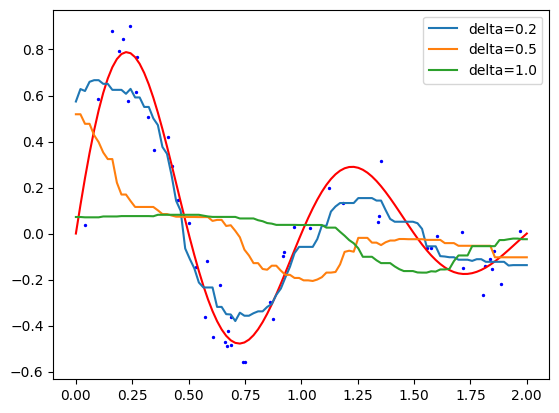
\includegraphics[scale=0.6]{img/kmeans_smoother.png}
      \caption{K means smoother} 
      \label{fig:kmeans_smoother}
    \end{figure}
  \end{example}

  \begin{code}[MWS of K Nearest Neighbor Regression in scikit-learn]
    Local averaging is implemented as the K nearest neighbor regressor in scikit learn. It is slightly different in the way that it doesn't use the points within a certain $\delta$ away but rather the $K$ nearest points. Either way, a minimal working example of this is 
    \begin{lstlisting}
      X = [[0], [1], [2], [3]]
      y = [0, 0, 1, 1]
      from sklearn.neighbors import KNeighborsRegressor
      neigh = KNeighborsRegressor(n_neighbors=2)
      neigh.fit(X, y)
      print(neigh.predict([[1.5]])) 
    \end{lstlisting}
  \end{code}

  Note that since $\hat{f}$ is a combination of step functions, this makes it discontinuous at points. 

\section{Kernel Regression and Linear Smoothers} 

  K nearest neighbor regression puts equal weights on both near and far points, as long as they are in the window. This may not be ideal, so a simple modification is to \textit{weigh} these points according to their distance from the middle $x$. We can do this with a kernel, as the name suggests. Now this is not the same thing as a Mercer kernel in RKHS, so to distinguish that I will call it a \textit{local averaging kernel}. 

  \begin{definition}[Local Averaging Kernel]
    A \textbf{kernel} is any smooth, symmetric, and non-negative function $K : \mathbb{R} \to \mathbb{R}$.  
  \end{definition}

  \begin{definition}[Kernel Regression]
    Given some datapoints, $X$, our fitted regressor is of form 
    \begin{equation}
      \hat{f} (X) = \frac{\sum_{i} Y_i K \bigg( \frac{||X - X_i||}{h} \bigg)}{\sum_{i} K \bigg( \frac{||X - X_i||}{h} \bigg)}
    \end{equation}
    where $h$ is the \textbf{bandwidth} and the denominator is made sure so that the coefficients sum to $1$. To get a clearer picture, we are really taking the weighted average of the $Y_i$'s. 
    \begin{equation}
      \hat{f} (X) = \sum_{i} Y_i \ell_i (X) \text{ where } \sum_{i} \ell_i (X) = 1
    \end{equation}
    Denoting $Y = (Y_1, \ldots, Y_n) \in \mathbb{R}^n$ and the vector $f(X) = (f(X_1), \ldots, f(X_n))$, if we can write the kernel function as $\hat{Y} = \hat{f}(X) = S Y$, which in matrix form, is 
    \begin{equation}
      \begin{bmatrix} \hat{Y}_1 \\ \vdots \\ \hat{Y}_n \end{bmatrix} = \begin{bmatrix} \hat{f}(X_1) \\ \vdots \\ \hat{f} (X_n) \end{bmatrix} = \begin{bmatrix} \ell_1 (X_1) & \cdots & \ell_n (X_1) \\ \vdots & \ddots & \vdots \\ \ell_1 (X_n) & \cdots & \ell_n (X_n) \end{bmatrix} \begin{bmatrix} Y_1 \\ \vdots \\ Y_n \end{bmatrix} 
    \end{equation}
    then we say that we have a \textbf{linear smoother}, with stochastic matrix $S$ being our \textbf{smoothing matrix}. 
  \end{definition}

  The reason we'd like to have the weights to sum to $1$ is that if we had data that was constant (i.e. all $Y_i$'s are the same), then the fitted function should be constant at that value as well. Furthermore, the theme of linearity is important and will be recurring. The kernel estimator is defined for all $X$, but it's important to see its behavior at the training points $X_i$. The estimator $\hat{Y} = \hat{f}(X)$ is a linear combination of the $Y_i$'s, and the coefficients $\ell_i (X_j)$ depend on the values of $X_j$. Therefore, we have $\hat{Y} = S Y$, which is very similar to the equation $\hat{Y} = H Y$ in linear regression, where $H$ is the hat matrix that projects $Y$ onto the column space of $X$. Nonparametric regression has the same form, but rather than being a projection, it is a linear smoothing matrix. Therefore, this theme unifies both linear regression and nonparametric regression. Linear smoothers, spline smoother, Gaussian processes, are all just different choices of the smoothing matrix $S$. However, not all nonparametric estimators are linear smoothers, as we will see later. 

  Here are some popular kernels. 

  \begin{definition}[Gaussian Kernel]
    The \textbf{Gaussian kernel} is defined as 
    \begin{equation}
      K(x) = \frac{1}{\sqrt{2 \pi}} e^{-x^2/2}
    \end{equation}
    \begin{figure}[H]
      \centering 
      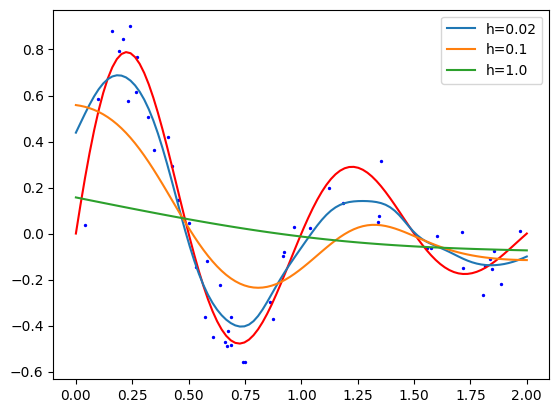
\includegraphics[scale=0.6]{img/gaussian_smoother.png}
      \caption{Gaussian kernel. } 
      \label{fig:gaussian_smoother}
    \end{figure}
  \end{definition}

  \begin{definition}[Box-Car Kernel]
    The \textbf{Box-Car kernel} is defined as 
    \begin{equation}
      K(x) = \frac{1}{2} \mathbbm{1}(|x| \leq 1)
    \end{equation}
    \begin{figure}[H]
      \centering 
      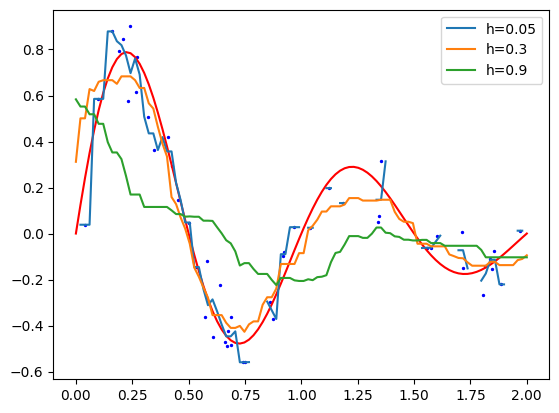
\includegraphics[scale=0.6]{img/boxcar_smoother.png}
      \caption{Boxcar kernel. } 
      \label{fig:boxcar_smoother}
    \end{figure}
  \end{definition}

  \begin{definition}[Epanechnikov Kernel]
    The \textbf{Epanechnikov kernel} is defined as 
    \begin{equation}
      K(x) = \frac{3}{4} (1 - x^2) \mathbbm{1}(|x| \leq 1)
    \end{equation}
    \begin{figure}[H]
      \centering 
      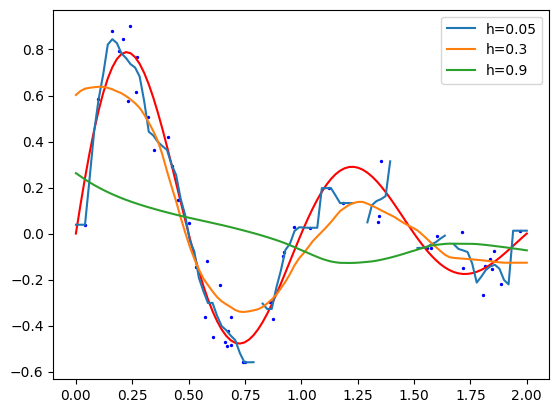
\includegraphics[scale=0.6]{img/epanechnikov_smoother.png}
      \caption{Epanechnikov kernel.} 
      \label{fig:epanechnikov_smoother}
    \end{figure}
  \end{definition}

  It turns out that from a theoretical point of view, the choice of the kernel doesn't really matter. What really matters is the bandwidth $h$ since that is what determines the bias variance tradeoff. To see why, if $h = 0$, then it will simply interpolate the points and variance is extremely high, and if $h = \infty$, then the fitted function will be constant at $\bar{Y}$, leading to high bias. The following theorem formalizes this.  

  \begin{theorem}[Bias Variance Tradeoff of Kernel Regression]
    Suppose that $d = 1$ and that $m^{\prime\prime}$ is bounded. Also suppose that $X$ has a nonzero, differentiable density $p$ and that the support is unbounded. Then, the risk is 
    \begin{align}
      R_n & = \frac{h_n^4}{4} \bigg( \int x^2 K(x) \bigg)^2 \int \bigg( m^{\prime\prime} (x) + 2m^\prime (x) \frac{p^\prime (x)}{p(x)} \bigg)^2 \,dx \\
          & \;\;\; + \frac{\sigma^2 \int K^2(x)\,dx} {n h_n} \int \frac{dx}{p(x)} + o \bigg( \frac{1}{n h_n} \bigg) + o(h_n^4) 
    \end{align}
    The first term is the squared bias and the second term is the variance. 
  \end{theorem}
  \begin{proof}
    We first denote 
    \begin{equation}
      \hat{f}(X) = \frac{\frac{1}{nh} \sum_{i=1}^n K \bigg( \frac{X - X_i}{h} \bigg) Y_i}{\frac{1}{nh} \sum_{i=1}^n K \bigg( \frac{X - X_i}{h} \bigg)} 
    \end{equation}
    where the denominator is the kernel density estimator $\hat{p}(X)$. Therefore, we rewrite
    \begin{align}
      \hat{f} (x) - f(x) & = \frac{\hat{a}(x)}{\hat{p}(x)} - f(x) \\
                         & = \bigg( \frac{\hat{a}(x)}{\hat{p}(x)} - f(x) \bigg) \bigg( \frac{\hat{p}(x)}{p(x) + 1 - \frac{\hat{p}(x)}{p(x)}} \bigg) \\
                         & = \frac{\hat{a}(x) - f(x) \hat{p}(x)}{p(x)} + \frac{(\hat{f}(x) - f(x)) (p(x) - \hat{p}(x))}{p(x)}
    \end{align}
    as $n \rightarrow \infty$ both $\hat{f}(x) - f(x)$ and $p(x) - \hat{p}(x)$ going to $0$, and since they're multiplied in the second term, it will go to $0$ very fast. So the dominant term is the first term, and we can write the above as approximately 
    \begin{equation}
      \hat{f}(x) - f(x) \approx  \frac{\hat{a}(x) - f(x) \hat{p}(x)}{p(x)}
    \end{equation}
    TBD continued. Wasserman lecture 6, 10:00. 
  \end{proof}

  From the theorem above, we can see that if the bandwidth is small, then $h^4$ is small and the bias decreases. However, there is a $h$ term in the denominator of the variance term, which also trades it off. We can furthermore see that the bias is sensitive to $p^\prime / p(x)$. This means that if the density is steep, then the bias will be high. This is known as \textit{design bias}, which is an underlying weakness in smoothing kernel regression. Another problem that is not contained in the theorem is the \textit{boundary bias}, which states that if you're near the boundary of the distribution (i.e. near the boundary of its support), then the bias also explodes. This happens to be very nasty especially in high dimensions where most of the data tends to be near the boundary. It turns out that this can be easily fixed with local polynomial regression, which gets rid of this term in the bias without any cost to variance. This means that this is unnecessary bias. 

  Then you can apply regularization on this to get kernel ridge regression. 

  \begin{code}[MWS of Kernel Ridge Regression in scikit learn]
    \begin{lstlisting}
      from sklearn.kernel_ridge import KernelRidge
      import numpy as np
      n_samples, n_features = 10, 5
      rng = np.random.RandomState(0)
      y = rng.randn(n_samples)
      X = rng.randn(n_samples, n_features)
      krr = KernelRidge(alpha=1.0)
      krr.fit(X, y)
    \end{lstlisting}
  \end{code}

\section{Local Polynomial Regression}

  Now another way to think about the kernel estimator is as such. Suppose that you're doing linear regression on a bunch of points and you want to choose a $c$ that minimizes the loss. 
  \begin{equation}
    \sum_i (Y_i - c)^2
  \end{equation}
  You would just pick $c = \hat{Y}$. But if you are given some sort of locality condition, that the value of $c$ should depend more on the values closer to it, you're really now minimizing 
  \begin{equation}
    \sum_i (Y_i - c(x))^2 K \bigg( \frac{X_i - x}{h} \bigg)
  \end{equation}
  Minimizing this by setting the derivative equal to $0$ and solving gives us the kernel estimator. Therefore you're fitting some sort of local constant at a point $X$. But why fit a local constant, when you can fit a local line or polynomial? This is the idea behind local polynomial regression.

  \begin{figure}[H]
    \centering 
    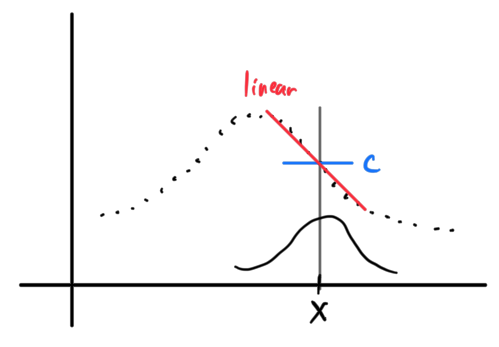
\includegraphics[scale=0.4]{img/local_linear_estimator.png}
    \caption{Rather than using a local constant, we can use a local linear estimator.} 
    \label{fig:local_linear_estimator}
  \end{figure}

  Therefore, we can minimize the modified loss. 

  \begin{definition}[Local Polynomial Estimator]
    The \textbf{local polynomial estimator} is a local linear kernel smoother that estimates the function $\hat{f}$ that minimizes the following loss. 
    \begin{equation}
      \argmin_{\beta} \sum_i K \bigg( \frac{X_i - x}{h} \bigg) \big( Y_i - (\beta_0 (x) - \beta_1 (x) (x- X_i) + \ldots + \beta_k (x) (x - X_i)^k )\big)
    \end{equation}
  \end{definition}

  So we can fit a line 
  \begin{equation}
    f(\mu) \approx \hat{\beta}_0 (x) + \hat{\beta}_1 (x) (\mu - x)
  \end{equation}
  and simply remove the intercept term to get the local linear estimator. 
  \begin{equation}
    \hat{f}(x) = \hat{\beta}_0 (x)
  \end{equation}
  Note that this is not the same as taking the constant estimate. We are extracting the fitted intercept term and so $\hat{\beta}_0(x) \neq c(x)$. 

  \begin{theorem}[Weighted Least Squares]
    The solution to the local linear estimator is similar to the weighted least squares solution. 
    \begin{equation}
      \hat{\beta}(x) = \begin{pmatrix} \hat{\beta}_0 (x) \\ \hat{\beta}_1 (x) \end{pmatrix} = (X^T W X)^{-1} X^T W Y
    \end{equation}
    where 
    \begin{equation}
      X = \begin{pmatrix} 1 & X_1 - x \\ \vdots & \vdots \\ 1 & X_n - x \end{pmatrix} \qquad W = \begin{pmatrix} K \bigg( \frac{X_1 - x}{h} \bigg) & 0 & \cdots & 0 \\ 0 & K \bigg( \frac{X_2 - x}{h} \bigg) & \cdots & 0 \\ \vdots & \vdots & \ddots & \vdots \\ 0 & 0 & \cdots & K \bigg( \frac{X_n - x}{h} \bigg) \end{pmatrix}
    \end{equation}
  \end{theorem}

  Computationally, it's similar to kernel regression and it gets rid of both the boundary and design bias. 

\section{Regularized: Spline Smoothing}

  This is not local, but it's a linear smoother. 

\section{Regularized: RKHS Regression}

  This is not local, but it's a linear smoother. 

\section{Additive Models}

  In the most general case, we want to create nonparametric regression functions of the form 
  \begin{equation}
    Y = f(x_1, \ldots, x_d) + \epsilon 
  \end{equation}
  We've done this for one dimensional case, but we can extend this to multiple dimensions through additive models of the form 
  \begin{equation}
    Y = \sum_j f_j (x_j)  + \epsilon
  \end{equation}
  This gives us very interpretable models where we can clearly see the effect of each covariate on $Y$. Clearly, this is not as flexible as the previous model since they can't capture dependencies, but we can create sub-dependency functions and replace the form above to something like 
  \begin{equation}
    Y = \sum_{i, j} f_{i, j} (x_i, x_j) + \epsilon
  \end{equation}
  giving us more flexible models. 

\section{Nonlinear Smoothers, Trend Filtering} 

  Tough example of the Dobbler function (like topologists sine curve). It's a pretty good fit but it's not too good since it's using a linear smoother (homogeneous). So we might need to fit it with nonlinear smoothers. 

\bibliography{./bibfile}
\bibliographystyle{alpha}

\end{document}
